\section{GNU Radio}


\subsection{Flowgraphs}

GNU Radio implements a dataflow system, where blocks are used to process data. Blocks receive several samples at once in their input buffers, process them and place the result in their output buffer. There are two important ways to pass data from one block to another: streams and message passing.
\paragraph*{Streams}
Streams are the most common way to transmit signal data between blocks. A stream is an endless sequence of samples which have a certain data type. Data types can be distinguished by color, as illustrated in \reff{gnuradio_block}.

\begin{figure}[H]
    \centering
    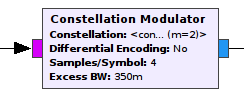
\includegraphics[width=0.3\textwidth]{img_other/gnuradio_block.png}
    \caption{{A GNU Radio block that gets a byte stream as input and outputs complex symbols} }
    \label{fig:gnuradio_block}
\end{figure}

Many data types exist in GNU Radio, but only a few are used in practice. Complex samples are blue, floats are orange and bytes are purple.
\begin{figure}[H]
    \centering
    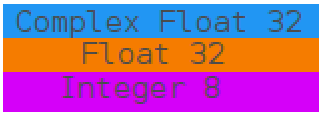
\includegraphics[width=0.25\textwidth]{img_other/datatypes.png}
    \label{fig:datatypes}
\end{figure}

\paragraph*{Tagged streams}
Tagged data streams are an extension of data streams. A tag can be attached to a stream sample, and provides extra control information. Tags are useful to transmit indicators, for example the start and length of a packet.
\begin{figure}[H]
    \centering
    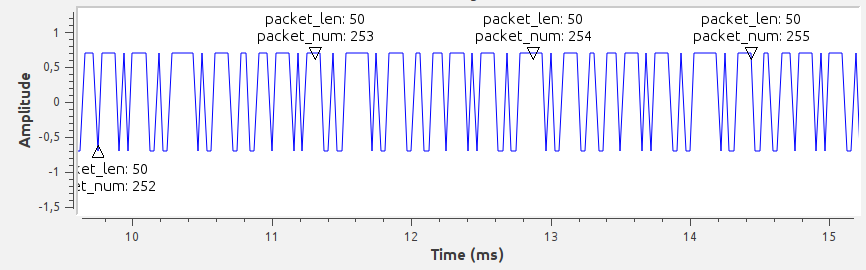
\includegraphics[width=0.95\textwidth]{img_other/tagged_streams.png}
    \caption{Stream tags to indicate the packet start, length and sequence number}
    \label{fig:datatypes}
\end{figure}



\paragraph*{Message passing}
Message passing is a more recent feature, and particularly useful to transmit control and meta data. In contrast to data streams, message passing blocks can be connected to upstream blocks in order to create feedback loops. A message connection is indicated with a dotted line, instead of a solid line.

\subsection{Block development in GNU Radio}
Users can build new Out-of-Tree modules containing new blocks to add extra functionality to the framework.  These blocks are developed in C++ or Python, where C++ focuses on performance and Python on ease of development. A special type of block is a \textit{hier} block, which is a block that internally connects several existing blocks. They can be used to quickly turn existing systems into a separate entity which can be integrated in larger systems.\medskip

We implemented several blocks in this semester project. Technical software development details are not given since block development relies heavily on the GNU Radio API, which can be found online \cite{gr_doxygen}.


